%%% The main file. It contains definitions of basic parameters and includes all other parts.

%% Settings for single-side (simplex) printing
% Margins: left 40mm, right 25mm, top and bottom 25mm
% (but beware, LaTeX adds 1in implicitly)
\documentclass[12pt,a4paper]{report}
\setlength\textwidth{145mm}
\setlength\textheight{247mm}
\setlength\oddsidemargin{15mm}
\setlength\evensidemargin{15mm}
\setlength\topmargin{0mm}
\setlength\headsep{0mm}
\setlength\headheight{0mm}
% \openright makes the following text appear on a right-hand page
\let\openright=\clearpage

%% Settings for two-sided (duplex) printing
% \documentclass[12pt,a4paper,twoside,openright]{report}
% \setlength\textwidth{145mm}
% \setlength\textheight{247mm}
% \setlength\oddsidemargin{14.2mm}
% \setlength\evensidemargin{0mm}
% \setlength\topmargin{0mm}
% \setlength\headsep{0mm}
% \setlength\headheight{0mm}
% \let\openright=\cleardoublepage


% All packages are imported here

%% Generate PDF/A-2u
\usepackage[a-2u]{pdfx}

%% Character encoding: usually latin2, cp1250 or utf8:
\usepackage[utf8]{inputenc}

%% Prefer Latin Modern fonts
\usepackage{lmodern}

%% Further useful packages (included in most LaTeX distributions)
\usepackage{amsmath}        % extensions for typesetting of math
\usepackage{amsfonts}       % math fonts
\usepackage{amsthm}         % theorems, definitions, etc.
\usepackage{bbding}         % various symbols (squares, asterisks, scissors, ...)
\usepackage{bm}             % boldface symbols (\bm)
\usepackage{graphicx}       % embedding of pictures
\usepackage{fancyvrb}       % improved verbatim environment
%\usepackage{natbib}         % citation style AUTHOR (YEAR), or AUTHOR [NUMBER]
\usepackage[nottoc]{tocbibind} % makes sure that bibliography and the lists
			    % of figures/tables are included in the table
			    % of contents
\usepackage{dcolumn}        % improved alignment of table columns
\usepackage{booktabs}       % improved horizontal lines in tables
\usepackage{paralist}       % improved enumerate and itemize
\usepackage{xcolor}         % typesetting in color

\usepackage[toc,acronym]{glossaries}
%%% Basic information on the thesis

% Thesis title in English (exactly as in the formal assignment)
\def\ThesisTitle{GPU Parallelization of Evolutionary Algorithms}

% Author of the thesis
\def\ThesisAuthor{Patrik Valkovič}

% Year when the thesis is submitted
\def\YearSubmitted{2021}

% Name of the department or institute, where the work was officially assigned
% (according to the Organizational Structure of MFF UK in English,
% or a full name of a department outside MFF)
\def\Department{Department of Theoretical Computer Science and Mathematical Logic}

% Is it a department (katedra), or an institute (ústav)?
\def\DeptType{Department}

% Thesis supervisor: name, surname and titles
\def\Supervisor{Mgr. Martin Pilát, Ph.D.}

% Supervisor's department (again according to Organizational structure of MFF)
\def\SupervisorsDepartment{Department of Theoretical Computer Science and Mathematical Logic}

% Study programme and specialization
\def\StudyProgramme{Computer Science}
\def\StudyBranch{Artificial Intelligence}

% Abstract (recommended length around 80-200 words; this is not a copy of your thesis assignment!)
\def\Abstract{%
\acrlongpl*{acc:gpu} stand for the success of \acrlong*{acc:ai} over the last decade and their broader application in the industry. Another promising field of \acrlong*{acc:ai} is \acrlong*{acc:ea}. Their parallelization ability is well known and has been successfully applied in practice. However, these attempts focused on multi--core and multi--machine parallelization rather than on the \acrshort*{acc:gpu}.\\
This work explores the possibilities of \acrlong*{acc:ea} parallelization on \acrshort*{acc:gpu}. I propose implementation in PyTorch library, allowing execution of \acrshort*{acc:ea} on \acrshort*{acc:gpu}. The proposed implementation provides the most common evolutionary operators for \acrlongpl*{acc:ga}, Real--Coded Evolutionary Algorithms, and \acrlong*{acc:pso} Algorithms. Finally, I show the performance is by order of magnitude faster on \acrshort*{acc:gpu} for medium and big--sized problems and populations.
}

% 3 to 5 keywords (recommended), each enclosed in curly braces
\def\Keywords{%
{Evolutionary Algorithms}, {Parallelization}, {GPU Computing}, {Genetic Algorithms}, {Particle Swarm Optimization}
}
% An optional dedication: you can thank whomever you wish (your supervisor,
% consultant, a person who lent the software, etc.)
\def\Dedication{%
I wish to thank my supervisor, Mgr. Martin Pilát, Ph.D., for his guidance, help, and mostly patience during my work on this thesis. I am thankful for his friendly attitude and valuable advice.

I would also want to express my sincere gratitude to my family and friends, without which support this work would not have been possible.

Computational resources were supplied by the project "e-Infrastruktura CZ" (e-INFRA LM2018140) provided within the program Projects of Large Research, Development and Innovations Infrastructures.
I would like to thank Cesnet for allowing me to use the computational power of MetaCentrum for the purpose of this thesis. I could not get presented results without their support.
}
%%% This file contains definitions of various useful macros and environments %%%
%%% Please add more macros here instead of cluttering other files with them. %%%

%%% Minor tweaks of style

% These macros employ a little dirty trick to convince LaTeX to typeset
% chapter headings sanely, without lots of empty space above them.
% Feel free to ignore.
\makeatletter
\def\@makechapterhead#1{
  {\parindent \z@ \raggedright \normalfont
   \Huge\bfseries \thechapter. #1
   \par\nobreak
   \vskip 20\p@
}}
\def\@makeschapterhead#1{
  {\parindent \z@ \raggedright \normalfont
   \Huge\bfseries #1
   \par\nobreak
   \vskip 20\p@
}}
\makeatother

% This macro defines a chapter, which is not numbered, but is included
% in the table of contents.
\def\chapwithtoc#1{
\chapter*{#1}
\addcontentsline{toc}{chapter}{#1}
}

% Draw black "slugs" whenever a line overflows, so that we can spot it easily.
\overfullrule=1mm

%%% Macros for definitions, theorems, claims, examples, ... (requires amsthm package)

\theoremstyle{plain}
\newtheorem{thm}{Theorem}
\newtheorem{lemma}[thm]{Lemma}
\newtheorem{claim}[thm]{Claim}

\theoremstyle{plain}
\newtheorem{defn}{Definition}

\theoremstyle{remark}
\newtheorem*{cor}{Corollary}
\newtheorem*{rem}{Remark}
\newtheorem*{example}{Example}

%%% An environment for proofs

\newenvironment{myproof}{
  \par\medskip\noindent
  \textit{Proof}.
}{
\newline
\rightline{$\qedsymbol$}
}

%%% An environment for typesetting of program code and input/output
%%% of programs. (Requires the fancyvrb package -- fancy verbatim.)

\DefineVerbatimEnvironment{code}{Verbatim}{fontsize=\small, frame=single}

%%% The field of all real and natural numbers
\newcommand{\R}{\mathbb{R}}
\newcommand{\N}{\mathbb{N}}

%%% Useful operators for statistics and probability
\DeclareMathOperator{\pr}{\textsf{P}}
\DeclareMathOperator{\E}{\textsf{E}\,}
\DeclareMathOperator{\var}{\textrm{var}}
\DeclareMathOperator{\sd}{\textrm{sd}}

%%% Transposition of a vector/matrix
\newcommand{\T}[1]{#1^\top}

%%% Various math goodies
\newcommand{\goto}{\rightarrow}
\newcommand{\gotop}{\stackrel{P}{\longrightarrow}}
\newcommand{\maon}[1]{o(n^{#1})}
\newcommand{\abs}[1]{\left|{#1}\right|}
\newcommand{\dint}{\int_0^\tau\!\!\int_0^\tau}
\newcommand{\isqr}[1]{\frac{1}{\sqrt{#1}}}

%%% Various table goodies
\newcommand{\pulrad}[1]{\raisebox{1.5ex}[0pt]{#1}}
\newcommand{\mc}[1]{\multicolumn{1}{c}{#1}}

\newcommand{\defterm}[1]{\vspace{0.6em}\noindent\textbf{#1}}

\newcommand{\individual}{\pmb{p}}
\newcommand{\population}{\mathcal{P}}
\newcommand{\fitnessfn}{f_f}
\newcommand{\objectivefn}{f_o}

\DeclareMathOperator*{\argmax}{arg\,max}
\DeclareMathOperator*{\argmin}{arg\,min}
\newcommand{\norm}[1]{\left\lVert#1\right\rVert}

\newcommand{\snipescondition}{increase variety of the population}
\makeglossaries

\newacronym{acc:ann}{ANN}{Artificial Neural Networks}
\newacronym{acc:ai}{AI}{Artificial intelligence}
\newacronym{acc:dann}{DANN}{Deep Artificial Neural Networks}
\newacronym{acc:cnn}{CNN}{Convolutional Neural Networks}
\newacronym[plural=GPUs,firstplural=Graphical Processing Units (GPUs)]{acc:gpu}{GPU}{Graphical Processing Unit}
\newacronym{acc:tpu}{TPU}{Tensor Processing Unit}
\newacronym{acc:cuda}{CUDA}{Compute Unified Device Architecture}
\newacronym[plural=EAs]{acc:ea}{EA}{Evolutionary Algorithms}
\newacronym[plural=GAs, firstplural=Genetic Algorithms]{acc:ga}{GA}{Genetic Algorithm}
\newacronym{acc:es}{ES}{Evolution Strategies}
\newacronym{acc:pso}{PSO}{Particle Swarm Optimization}
\newacronym{acc:dna}{DNA}{Deoxyribonucleic Acid}
\newacronym{acc:tsp}{TSP}{Traveling Salesman Problem}
\newacronym{acc:blx}{BLX}{Blend Crossover}
\newacronym{acc:cma}{CMA--ES}{Covariance Matrix Adaptation -- Evolution Strategy}
\newacronym{acc:de}{DE}{Differential evolution}
\newacronym{acc:spso2006}{SPSO--2006}{Standard Particle Swarm Optimization 2006}  
\newacronym{acc:spso2011}{SPSO--2011}{Standard Particle Swarm Optimization 2011}  
\newacronym[plural=CPUs,firstplural=Central Processing Units (CPUs)]{acc:cpu}{CPU}{Central Processing Unit}
\newacronym{acc:ghz}{GHz}{gigahertz}
\newacronym{acc:mhz}{MHz}{megahertz}
\newacronym[plural=APIs,firstplural=Application Programming Interfaces (APIs)]{acc:api}{API}{Application Programming Interface}
\newacronym[plural=SMs, firstplural=Stream Multiprocessors]{acc:sm}{SM}{Stream Multiprocessor}
\newacronym[plural=SPs, firstplural=Stream Processors]{acc:sp}{SP}{Stream Processor}
\newacronym{acc:simd}{SIMD}{Single Instruction, Multiple Data}
\newacronym{acc:os}{OS}{Operating System}
\newacronym{acc:bbob}{BBOB}{Black--Box Optimization Benchmarking}
\newacronym{acc:coco}{COCO}{Comparing Continuous Optimizers}
\newacronym{acc:ffeat}{FFEAT}{Framework For Evolution Algorithms in Torch}
\newacronym{acc:sus}{SUS}{Stochastic Universal Sampling}
\newacronym{acc:sat}{SAT}{Boolean Satisfiability Problem}
\newacronym{acc:3sat}{3SAT}{\acrshort{acc:sat} problems with exactly three literals in clause}

%% The hyperref package for clickable links in PDF and also for storing
%% metadata to PDF (including the table of contents).
%% Most settings are pre-set by the pdfx package.
\hypersetup{unicode}
\hypersetup{breaklinks=true}

% Title page and various mandatory informational pages
\begin{document}
%%% Title page of the thesis and other mandatory pages

%%% Title page of the thesis

\pagestyle{empty}
\hypersetup{pageanchor=false}
\begin{center}

\centerline{\mbox{
\includegraphics[width=166mm]{img/logo-en.pdf}}}

\vspace{-8mm}
\vfill

{\bf\Large MASTER THESIS}

\vfill

{\LARGE\ThesisAuthor}

\vspace{15mm}

{\LARGE\bfseries\ThesisTitle}

\vfill

\Department

\vfill

{
\centerline{\vbox{\halign{\hbox to 0.45\hsize{\hfil #}&\hskip 0.5em\parbox[t]{0.45\hsize}{\raggedright #}\cr
Supervisor of the master thesis:&\Supervisor \cr
\noalign{\vspace{2mm}}
Study programme:&\StudyProgramme \cr
\noalign{\vspace{2mm}}
Study branch:&\StudyBranch \cr
}}}}

\vfill

% Zde doplňte rok
Prague \YearSubmitted

\end{center}

\newpage

%%% Here should be a bound sheet included -- a signed copy of the "master
%%% thesis assignment". This assignment is NOT a part of the electronic
%%% version of the thesis. DO NOT SCAN.

%%% A page with a solemn declaration to the master thesis

\openright
\hypersetup{pageanchor=true}
\pagestyle{plain}
\pagenumbering{roman}
\vglue 0pt plus 1fill

\noindent
I declare that I carried out this master thesis independently, and only with the cited
sources, literature and other professional sources. It has not been used to obtain another
or the same degree.

\medskip\noindent
I understand that my work relates to the rights and obligations under the Act No.~121/2000 Sb.,
the Copyright Act, as amended, in particular the fact that the Charles
University has the right to conclude a license agreement on the use of this
work as a school work pursuant to Section 60 subsection 1 of the Copyright~Act.

\vspace{10mm}

\hbox{\hbox to 0.5\hsize{%
In \hbox to 6em{\dotfill} date \hbox to 6em{\dotfill}
\hss}\hbox to 0.5\hsize{\dotfill\quad}}
\smallskip
\hbox{\hbox to 0.5\hsize{}\hbox to 0.5\hsize{\hfil Author's signature\hfil}}

\vspace{20mm}
\newpage

%%% Dedication

\openright

\noindent
\Dedication

\newpage

%%% Mandatory information page of the thesis

\openright

\vbox to 0.5\vsize{
\setlength\parindent{0mm}
\setlength\parskip{5mm}

Title:
\ThesisTitle

Author:
\ThesisAuthor

\DeptType:
\Department

Supervisor:
\Supervisor, \SupervisorsDepartment

Abstract:
\Abstract

Keywords:
\Keywords

\vss}

\newpage

\openright
\pagestyle{plain}
\pagenumbering{arabic}
\setcounter{page}{1}


%%% A page with automatically generated table of contents of the master thesis
\setcounter{tocdepth}{1}
\tableofcontents
% TODO fix document outline to generate subsection and table of content as well

%%% Each chapter is kept in a separate file
\chapter{Introduction}

\acrfull{acc:ai} 
has become phenomenon of these days. Latest advances in this field achieved magnificent results and allowed creation of systems and tools, we though would be possible thirty years back. The biggest credit goes to the \acrfull{acc:ann}
, which allowed this rapid and astonishing growth of the field. More precisely, the \acrfull{acc:daan} 
sparkled this process in 2011, when they started to exceed human performance in German traffic sign recognition benchmark \cite{CIRESAN2012333}.
\chapter{\texorpdfstring{\acrlong*{acc:ea}}{}}

Optimization. What better word would describe the ultimate goal of all the people, our civilization, and maybe even the Universe. With a bit of exaggeration, optimization is the cause of all the ramifications we can see around. Because what else are Physic laws than minimization processes, our pursuit of knowledge and self improvement than maximization of self-worth, industrial revolutions than minimization of human labour, maximization of goods production and standard of living at the same time. In my opinion, optimization is the reason what drives us forward, makes us better, and guides our decisions.

One of the most extraordinary optimization processes is, without a doubt, evolution. Evolution is nothing less than Nature way of improvement species to better adapt to their environment. The father of evolution is undoubtedly Charles, who the first come up with an idea of evolution in his work \enquote{On the origin of species: A facsimile of the first edition} \citep{darwin1964origin}. According the him, the individuals that better adapted to the environment have higher potential to reproduce and pass their genetic material --- including the predisposition to survive in the environment --- to their offsprings. Sometimes referred as \enquote{Survival of the fittest}.

This exact ideas inspired scientists and formed the field of \acrfull{acc:ea}\index{evolutionary algorithm}\footnote{I will refer to all the population-based algorithms in this work as \acrlong*{acc:ea}. These includes, among others, \acrlong*{acc:ga}, \acrlong*{acc:ea}, and \acrlong*{acc:pso}.}.
\acrshort{acc:ea} are stochastic, population-based optimization algorithms inspired by biological evolution. In general, a set of individuals called population compete with each other for a place in the next generation. Each individual represent one possible solution of the problem in hand. Quality of the individual is proportional to the quality of solution it represents. This quality is usually expressed using fitness (or sometimes called objective) function. As with natural evolution, the probability of survival is proportional the solution quality -- the better the solution is, the higher the probability of survival \citep{IntroductionToEA}. In the \acrshort{acc:ea}, the process of producing new generation is usually called selection.

Evolution is not only about survival, but also about reproduction. \acrlong*{acc:ea} took inspiration here as well and uses specials operators for each generation -- usually called evolution operators or variation operators\index{variation operator}. As the name suggests, these operators make sure the population explores new solutions. The two most common operators are crossover and mutation. During crossover\index{crossover}, individuals from the current population (usually called parents) produces new individuals (usually called offsprings) by combining their genetic information. In some way, crossover mimic reproduction in Nature, during which the \acrshort{acc:dna} of offspring is by majority determined by its parents \acrshort{acc:dna}. Mutation\index{mutation}, on the other hand, causes random small alteration of the individual genetic material and is able to introduce novel patterns that did not previously occur in the population \citep{HowToSolveItModernHeuristics}.

In general, \acrshort{acc:ea} repeat steps above until sufficiently good solution is found, or until maximum number of generations is reached. The general pseudocode of the \acrshort{acc:ea} algorithm is in Algorithm \ref{alg:SEA}. I will present more accurate implementations of various algorithms thorough this chapter.

\begin{algorithm}
    \SetAlgoLined
    \KwResult{evolved population}
    initialize population\;
    \Repeat{termination criteria met}{
        reproduction\;
        mutation\;
        evaluate population\;
        selection\;
    }
    \caption{General Evolution Algorithm}
    \label{alg:SEA}
\end{algorithm}


%%%%%%%%%%%%%%%%%%%
%%               %%
%%  TERMINOLOGY  %%
%%               %%
%%%%%%%%%%%%%%%%%%%
\section{Terminology}

In this section, I will introduce necessary terminology that I am going to use thorough this work. I took most of the terminology from \citet{IntroductionToEA}.

\defterm{Problem} is the function we want to solve. It can be both satisfactory as well optimization problem.

\defterm{Genotype}\index{genotype} is encoding of the solution. It is equivalent of the \acrshort{acc:dna} -- it compress all the data needed to produce solution.

\defterm{Gene} is one part of the genotype. It may be one bit if the genotype is encoded as binary string or scalar, if the genotype is vector. 

\defterm{Representation or genotype space} is the space of genotype.

\defterm{Phenotype}\index{phenotype} is the solution built from genotype. Genotype and phenotype can be equivalent -- for example real function optimization problem may have as a genotype vector of real numbers, that represent one of the solution. Generally, however, genotype and phenotype can be different.

\defterm{Search space} is the space of phenotype.

\defterm{Objective function} is the function the algorithm optimize. For previous example of real function optimization, the function itself can be the objective function. I will denote objective function $\objectivefn$.

\defterm{Fitness function}\index{fitness function} is the measure of quality of the solution. Note that the domain of the function is the search space. Unlike the objective function, the fitness function should guide the algorithm during the optimization. It can use the objective function directly, but other options are possible as well. For example, if the goal is to maximize objective function $\objectivefn(x)$, but the algorithm is written such that it minimize the fitness function, one may specify the fitness function as $\fitnessfn(x)=\frac{1}{\objectivefn(x)}$. I will denote fitness function $\fitnessfn$.

\defterm{Evaluation} is the process of obtaining fitness value for the genotype.

\defterm{Individual} is genotype with it's fitness value. I will denote individual by $\individual$.

\defterm{Fitness value} of individual is it's evaluation. 

\defterm{Population} is multiset of individuals -- it is possible to have same genotype in the population multiple time. However, I will still distinguish different individuals with the same genotype. I will denote the whole population as $\population$.

\defterm{Initialization} is the process of creating the first population.

\defterm{Exploitation} is the effort to use knowledge from the history in order to maximize the expected outcome \citep{SelfAdaptiveFeaturesInRealParameterEvolutionaryAlgorithms}.

\defterm{Exploration} is the effort to discover new rules about the problem in hand, although the expected outcome does not need to be the best possible. In general, the biggest problem in \acrshort{acc:ea} is the right balance between exploitation and exploration. Putting too much emphasis may cause to get stuck in the local minima, whereas putting too much focus on the exploration may cause, that the algorithm never converge. Note that \acrshort{acc:ea} is not the only field suffering from this, but for example Reinforcement Learning deals with the same problems \citep{ExplorationExploitationDilemaRL}. 

\defterm{Evolution operators} are individual steps performed each iteration.

\defterm{Selection}\index{selection} is evolution operator that picks up individuals from the current population to the next one. The selection should take into account fitness of each individual in the population and pick them proportionally. Selection therefore implements the \enquote{Survival of the fittest} law. From the mathematical point of view, selection task is to move the population into more promising area of the search space and possibly to reduce variance of the population \citep{SelfAdaptiveFeaturesInRealParameterEvolutionaryAlgorithms}. In other word, selection is exploitation step in the algorithm.

\defterm{Crossover}\index{crossover} is evolution operator, that combines some individuals (usually called \textbf{parents}) in order to create one or more new individuals (usually called \textbf{offsprings}). Offsprings are usually combination of their parents, similarly to how \acrshort{acc:dna} of the child is combination of \acrshort{acc:dna} of her parents.

\defterm{Mutation}\index{mutation} is evolution operator, that modify one individual. Mutation can be based on randomness (for example replacement of value in genotype by different value) or specialized for the problem in hand. This time the example can be \acrlong{acc:tsp}, where one possible mutation operator can \enquote{untwist} ways that cross each other. This mutation is in fact local optimization technique, as the  mutated way is shorter than the previous one \citep{TSPArticle}.

\defterm{Variation operators}\index{variation operator} are operators, that change the variation of the population, but not the mean. Variation operators are the exploration steps in the algorithm and should balance the exploitation strength of the selection. Both crossover and mutation are variation operators \citep{SelfAdaptiveFeaturesInRealParameterEvolutionaryAlgorithms}.

\defterm{Memetic operator} is operator, that uses local optimization in every iteration. Alternatively, \enquote{memetic algorithms uses local optimizer to every solution before evaluation}\citep{HowToSolveItModernHeuristics}. One of such example is the \acrlong{acc:tsp} problem mentioned earlier. Another example is the problem of searching for weights in \acrshort{acc:ann}, where one step of backpropagation algorithm is performed as part of the mutation.




%%%%%%%%%%%%%%%%%%%%%%%%%%
%%                      %%
%%  GENETIC ALGORITHMS  %%
%%                      %%
%%%%%%%%%%%%%%%%%%%%%%%%%%
\section{\texorpdfstring{\acrlong*{acc:ga}}{}}

\acrfull{acc:ga} are probably the simplest \acrfull{acc:ea} out there and as their father is usually considered \citefullauthor{HollandGA}. In the \acrshort{acc:ga}, individual are binary string of length $n$, formally
$$ \individual \in \left\{0,1\right\}^{n} $$

Fitness function maps genotype into real values
$$ \fitnessfn:\left\{0,1\right\}^{n}\rightarrow\mathbb{R} $$

The typical crossover operator is one point crossover\index{crossover!one--point}. This type of crossover require two parents and produces two offsprings. As the first step, the algorithm uniformly sample random integer $s$ in the range $\left[ 1, n-1 \right]$. The first offspring will receive genetic material up to index $s$ from the first parent, and the rest from the second one. The second offspring is created the same way, except the position of parents is exchanged. Example for $n=10$ is in figure \ref{fig:gaonepointcrossover}. In order not to modify all the individuals in the population, only $p_c\in\left[0,1\right]$ percent of individuals undergo the crossover and the children replace their parents\citep{IntroductionToEA}.

\begin{figure}
    \begin{subfigure}[b]{0.4\textwidth}
        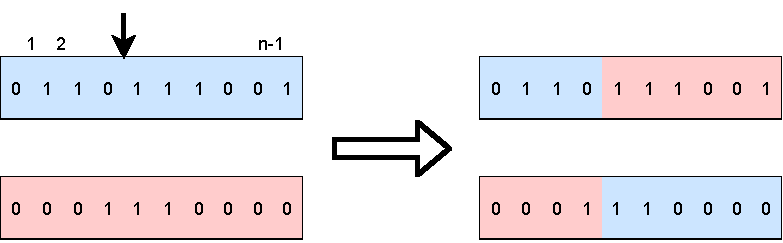
\includegraphics[width=\textwidth]{img/master_onepointcrossover.pdf}
        \caption{One point crossover}
        \label{fig:gaonepointcrossover}
    \end{subfigure}
    \hfill
    \begin{subfigure}[b]{0.4\textwidth}
        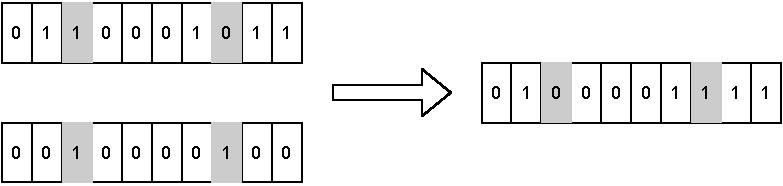
\includegraphics[width=\textwidth]{img/master_bitflipmutation.pdf}
        \caption{Bit-flip mutation}
        \label{fig:bitflipmutation}
    \end{subfigure}
    \caption{Genetic algorithm operators}
\end{figure}

The mutation\index{mutation} operator for \acrshort{acc:ga} is in most cases bit-flip mutation\index{mutation!bit-flip}. During this mutation, each gene in the genotype is mutated with probability $p_m$. One example of mutation is in figure \ref{fig:bitflipmutation}. Mutation has two objectives -- it makes sure the algorithm is not trapped in local optima, and it sustains genetic disparity in the population. As a side effect, mutation serves as minor search operator\citep{IntroToGA}.

The difference between crossover and mutation is such that crossover is rather \enquote{search} exploitation technique. It combines individuals from current population and exploit them to find possibly better individuals. Mutation, on the other hand, is more local search technique and based on the probability $p_b$ it search over the whole representation space.

Finally, the selection stage takes place. There are various selection techniques and in this particular case, I will use tournament selection\index{selection!tournament}. During tournament selection, fitness values of two random individuals are compared and the better individual is copied into the new population. This repeats as many times, as specified number of individuals form a new population.

For cases where the size of the new population equals to the size of the old one, there is high probability that the same individual will be in the following population multiple times. Nevertheless, because of crossover and mutation operators that doesn't matter, because they keep divergence in the population.

The pseudocode of simple genetic algorithm described above is depict in algorithm \ref{alg:SGA}. The population if firstly randomly initialized and then undergo crossover, mutation, evaluation, and selection operators in the loop. Finally, evolved population is returned from the algorithm.

\begin{algorithm}
    \KwIn{$d$ problem dimension, $l$ population size, $g$ generations, $\fitnessfn$, $p_c$, $p_m$}
    \KwResult{evolved population}
    population $\leftarrow$ randomly initialized\;
    \ForEach{$gen$ in $0$..$g$}{
        \ForEach{individual in $0$..$l$}{
            \If(){$rand()<p_c$}{One point crossover with random individual}
            \If(){$rand()<p_m$}{Bit-flip mutation}
        }
        Evaluate population using $\fitnessfn$\;
        population $\leftarrow$ pick up $l$ individuals using tournament\;
    }
    \Return{population}
    \caption{Simple genetic algorithm}
    \label{alg:SGA}
\end{algorithm}

I will refer to algorithm described above as \enquote{Simple Genetic Algorithm}. In reality, scientists come up with various operators, that can improve convergence or can help in specific types of problems. Thorough following paragraphs, I will focus on these techniques, inspired mainly by the book of authors \citet*{IntroToGA}.

%%  CROSSOVERS  %%
%%%%%%%%%%%%%%%%%%
\subsection{Advanced crossover operators}

Simple genetic algorithm used one point crossover. It is straightforward to extend it into two point crossover\index{crossover!two point} where each genome is split into three parts. Each offspring then receives first and third part of the genome from one parent, and the middle one from the second one. Example of two point crossover is in the picture \ref{fig:gatwopointcrossover}.

\begin{figure}
    \begin{subfigure}[b]{0.4\textwidth}
        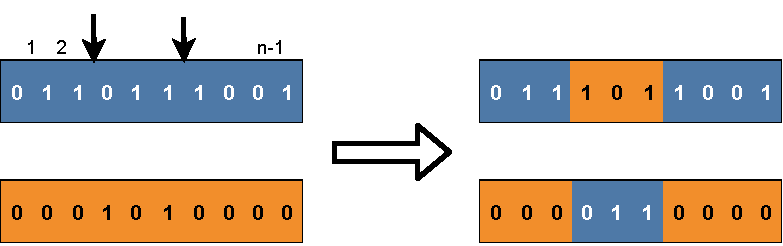
\includegraphics[width=\textwidth]{img/master_twopointcrossover.pdf}
        \caption{Two point crossover}
        \label{fig:gatwopointcrossover}
    \end{subfigure}
    \hfill
    \begin{subfigure}[b]{0.4\textwidth}
        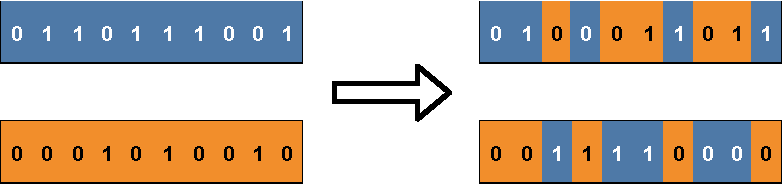
\includegraphics[width=\textwidth]{img/master_uniformcrossover.pdf}
        \caption{Uniform crossover}
        \label{fig:uniformcrossover}
    \end{subfigure}
    \caption{Advanced crossover operators}
\end{figure}

Sometimes, the crossover operator is generalized even more and forms $k$--point crossover. The genotype partitions into $k$ parts and these parts are interleaved in the offsprings. Special case is uniform crossover\index{crossover!uniform} -- the offsprings are constructed in such a way that they are uniform combination if their parents. Each gene in the offspring have equal probability whether it will be received from the first, or second parent. Second offspring will follow the same pattern, except with parents exchanged. Example of uniform crossover is in figure \ref{fig:uniformcrossover}.
% TODO Introduction into GA presents few more types - three parents crossover, crossover with reduced surrogate, and shuffle crossover. These are irrelevant for my implementation, but can be potentially described here.

I have described the crossover operators such that the offsprings replace their parents. That is a common design decision, however one does not need to enforce that and may decide to create offsprings in addition to the parents. To ensure the population does not increase in size, the selection operator can be implemented in a way that specified number of individuals will be picked up.

%%  SELECTION  %%
%%%%%%%%%%%%%%%%%
\subsection{Selection operators}


\chapter{Conclusion}
\label{chap:conclusion}

This work summarizes current knowledge of \acrlong*{acc:ea} and gives a comprehensive overview of this research field. It discusses the well--known evolutionary operators and gives their detailed analysis from the implementation point of view, along with their desired properties. The work further describes the three most common evolutionary algorithms -- the \acrlong{acc:ga}, real--\kern0.04em coded evolutionary algorithms, and the \acrlong{acc:pso} algorithms. Each of them is analyzed, and their representative operators are described and examined.

The work further discusses the differences between \cpu and \gpu and their architectures. I show that while the \gpu has its application in various fields mentioned in the work, the mindset for programming on \gpu is considerably different and unique. I present the OpenCL and \cuda technologies, and present the terminology used in \gpu programming. The work shows the elements of \cuda programming, with a particular focus on a performance issue that can arise. 

I then present the PyTorch library for the Python programming language, describe its architecture and functionality. The work put into connection the PyTorch library and \cuda programming discussed before. Follows discussion about possible ways to parallelize \acrlong{acc:ea} both on \cpu and \gpuns. The work focuses on different individual encoding, parallelization granularity, and evaluation architectures.

Follows presentation of the \acrfull{acc:ffeat}, my contribution to this area. I discuss in detail its functionality, implementation decisions, architecture, and the proposed workflow. The work gives extra space to challenging parts of the implementation, like parental sampling and crossover schemes. Some of these problems arise from the limitations of the PyTorch library and the \cuda programming in general; these aspects are discussed. Implementation of some operators is then shown in the text, and I discuss possible ways to extend the library. Overall, I show that the proposed implementation is easy to extend, operators are written in a readable manner and runs efficiently on \gpuns.

The implementation is subjected to extensive testing on \acrshort{acc:3sat} problem and \acrshort{acc:bbob} test suite. The experiments show the advantage of using \cuda implementation for medium and big--sized populations and problems. The experiments show an order of magnitude speedup using \cuda implementation rather than \cpuns. Moreover, the experiments show the advantage of a bigger population on some problems while leading to premature convergence on others. I discuss this phenomenon and explain the behavior of algorithms.

Finally, I compare the proposed implementation against the native \cpp implementation on the \acrshort{acc:3sat} problem. It shows a noticeable slowdown on one core machine but gets faster as the number of cores increases. The proposed implementation makes use of the parallelized operators implementation and becomes dominant. The comparison with \cpp implementation confirms the superiority of \cuda implementation for medium and big--sized populations.

This work dealt with \acrshort{acc:ga}, real--\kern0.04em coded evolutionary algorithms, and \acrshort{acc:pso} algorithms. There are other classes of algorithms that the implementation was not tested on. Further work could expand the library with these algorithms. I believe the \acrshort{acc:cma} would greatly benefit of \cuda implementation. Benchmark the implementation on permutation--based algorithms may seems interesting as well. Furthermore, all the presented problems have been vectorized, and the \gpu implementation could evaluate the whole population at once. It may be interesting to explore the possibility of evaluating each individual separately, taking away the major advantage of \gpu implementation. This may be practical for complicated fitness functions. Future work could explore this possibility and evaluate whether using \gpu implementation keeps its advantages.

%%% Bibliography
%%% Bibliography (literature used as a source)
%%%
%%% We employ bibTeX to construct the bibliography. It processes
%%% citations in the text (e.g., the \cite{...} macro) and looks up
%%% relevant entries in the bibliography.bib file.
%%%
%%% The \bibliographystyle command selects, which style will be used
%%% for references from the text. The argument in curly brackets is
%%% the name of the corresponding style file (*.bst). Both styles
%%% mentioned in this template are included in LaTeX distributions.

%\bibliographystyle{plainnat}   %% Author (year)
%\bibliographystyle{unsrt}      %% [number]
\bibliographystyle{apalike}    %% [Author, year]      

%\renewcommand{\bibname}{Bibliography}

%%% Generate the bibliography. Beware that if you cited no works,
%%% the empty list will be omitted completely.
\bibliography{bibliography,bibliographyintro}


%%% Figures used in the thesis (consider if this is needed)
\listoffigures

%%% Tables used in the thesis (consider if this is needed)
%%% In mathematical theses, it could be better to move the list of tables to the beginning of the thesis.
\listoftables

\listofalgorithms

%%% Abbreviations used in the thesis, if any, including their explanation
%%% In mathematical theses, it could be better to move the list of abbreviations to the beginning of the thesis.
%\chapwithtoc{List of Abbreviations}
\printglossary
\printglossary[type=\acronymtype, nonumberlist,title={List of Abbreviations}]

%%% Attachments to the master thesis, if any. Each attachment must be
%%% referred to at least once from the text of the thesis. Attachments
%%% are numbered.
%%%
%%% The printed version should preferably contain attachments, which can be
%%% read (additional tables and charts, supplementary text, examples of
%%% program output, etc.). The electronic version is more suited for attachments
%%% which will likely be used in an electronic form rather than read (program
%%% source code, data files, interactive charts, etc.). Electronic attachments
%%% should be uploaded to SIS and optionally also included in the thesis on a~CD/DVD.
%%% Allowed file formats are specified in provision of the rector no. 72/2017.
\appendix

\printindex

\chapter{Attachments}

\section{First Attachment} 
//TODO make sure attachments check

\openright
\end{document}
